\section{Exploración del tamaño de población}

\begin{table}[]
    \centering
    \begin{tabular}{||c|c|c|c|c|c||}
        \hline
        \textbf{Fichero Configuración} & \textbf{Generaciones} & \textbf{Tmñ. poblacion} & \textbf{Mejor fitness} & \textbf{Evals. de f}\\ \hline
        Config 1   & 18    & 100   & -47.80    &  2620   \\ \hline
        Config 7   & 43    & 150   & -25.39    &  9484   \\ \hline
        Config 8   & 57    & 300   & -30.94    &  26335  \\ \hline
        Config 9   & 65    & 500   & -33.30    &  49827  \\ \hline
        Config 10  & 75    & 1000  & -39.70    &  114611 \\ \hline
    \end{tabular}
    \caption{Resultados exploración inicial}
    \label{tab:base_population}
\end{table}

El objetivo de esta sección es obtener una población inicial base para las próximas exploraciones. Dejaremos fija la dimensión del cromosoma a 10 y
ejecutaremos cada fichero de configuración 15 veces. Se ha escogido esta dimensión porque ha alcanzado una solución 
relativamente buena en el experimento anterior; las 3 primeras las hemos descartado por su facilidad para encontrar un 
óptimo. Las soluciones de esta exploración se encuentran en la Tabla \ref{tab:base_population}. En esta nueva exploración se 
han probado los tamaños de población: 100, 150, 300, 500, 1000, indicados en la Tabla \ref{tab:base_population}
como \textit{Tmñ. poblacion}. Descartamos el tamaño 100 ya que tiene únicamente 18 generaciones, 15 de las cuales tienen el mismo
valor de fitness, lo que significa que se ha quedado estancado en un óptimo local a la tercera generación.

En la Figura \ref{fig:population_size_variation} se vuelve a ver cómo el mayor descenso del valor del fitness se produce
entre la generación 0 y la 20. La población con tamaño 300 (Config 8 en Tabla \ref{tab:base_population}) es la que tiene
un mayor descenso pasada la generación 20. 

\begin{figure}[]
	\centering	
	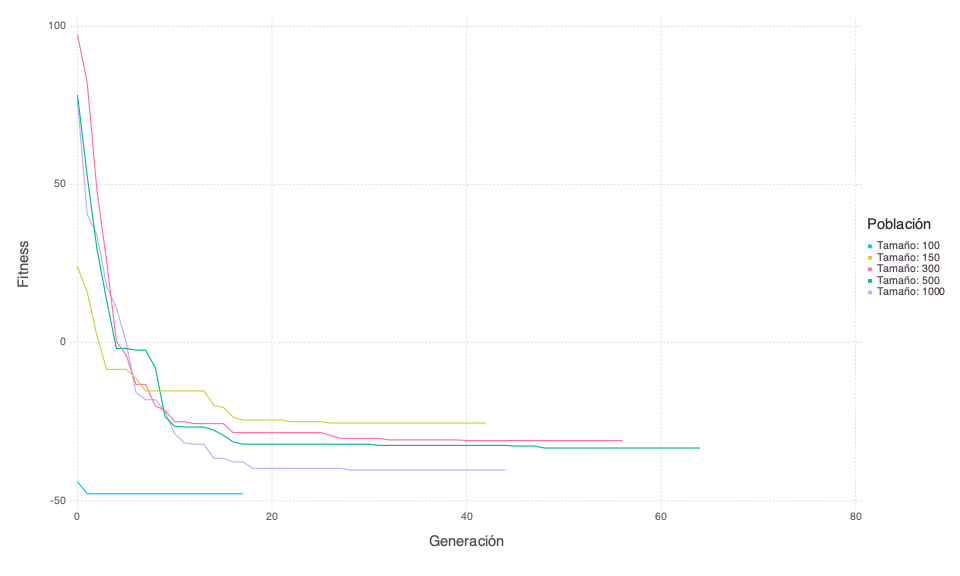
\includegraphics[scale=0.5]{figuras/population_size_variation.png}
	\caption{ Ejecuciones variando el tamaño de la población }
    \label{fig:population_size_variation}
\end{figure}

En la Figura \ref{fig:population_size_box_plots}, se puede ver que la Configuración 10, con tamaño de población 1000, es
la que tiene la distribución de valores más pequeños. Adicionalmente, es la que tiene también el mejor valor final, pero la
Figura \ref{fig:population_size_box_plots} confirma que no se trata de un caso atípico.

\begin{figure}[]
	\centering	
	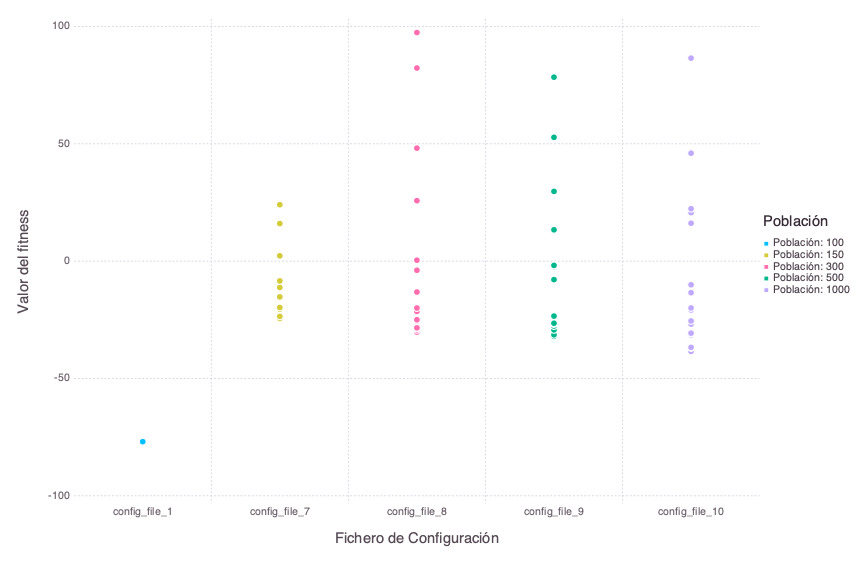
\includegraphics[scale=0.5]{figuras/Rastrigin_box_plots_p_size.png}
	\caption{ Diversidad en la ejecución variando el tamaño de población }
    \label{fig:population_size_box_plots}
\end{figure}


El objetivo de esta exploración era sacar una población inicial en la que basar el resto de experimentos. Si el criterio
es coger la que de mejor valor de fitness, entonces la mejor opción parece el tamaño de población 1000. Por confirmar que
esta es la decisión correcta, si añadimos como criterio la diversidad, la Figura \ref{fig:population_size_variation_diversity}
muestra cómo este tamaño de población mantiene mejor la diversidad con respecto al siguiente tamaño, con mejores 
resultados. En consecuencia, será la base del resto de experimentos.

\begin{figure}[]
	\centering	
	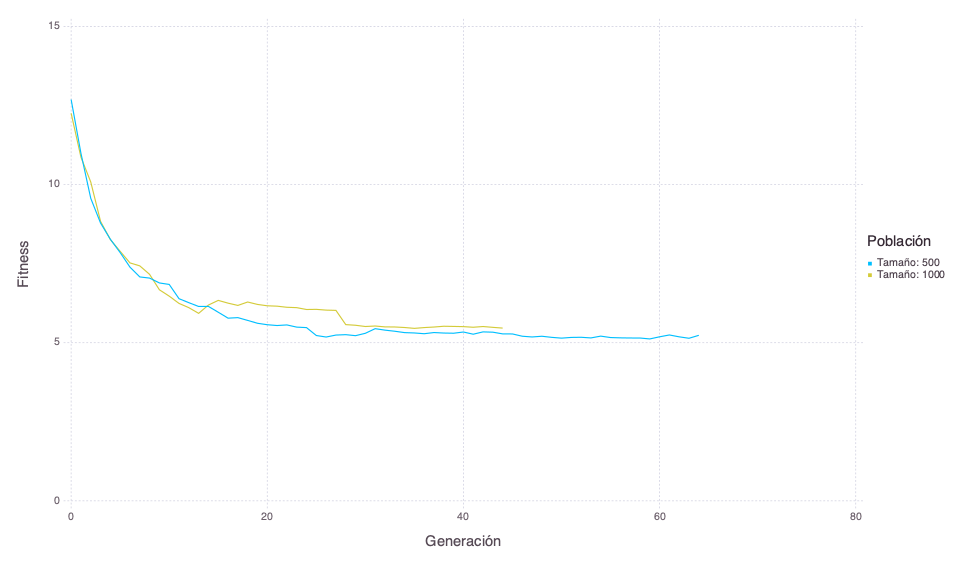
\includegraphics[scale=0.5]{figuras/population_size_variation_diversity.png}
	\caption{ Ejecuciones variando el tamaño de la población }
    \label{fig:population_size_variation_diversity}
\end{figure}
